%!TEX root = ../document.tex
\chapter{Buffer Overflow}
Buffer Overflow ist der Überbegriff für eine Schwachstelle im Quellcode der für einen Angriff genutzt wird und gehört zu den häufigsten Angriffsmethoden. Je nach Art der Schwachstelle wird auch von Heap-Overflow, Integer-Overflow oder String-Overflow gesprochen.
\section{Erklärung}
Einfach ausgedrückt, werden bei diesem Angriff einem Programm mehr Daten übergeben als es erwartet bzw. verarbeiten kann. Bei guter Programmierung führt dies zu einem Absturz des Programmes oder einer Fehlermeldung. Bei schlechter Programmierung (fehlender Überprüfung der Eingangsdaten) reicht der freigehaltene Speicherplatz für die Variable aber nicht aus und nachfolgende Speicherbereiche werden überschrieben.

\begin{figure}
	\centering
	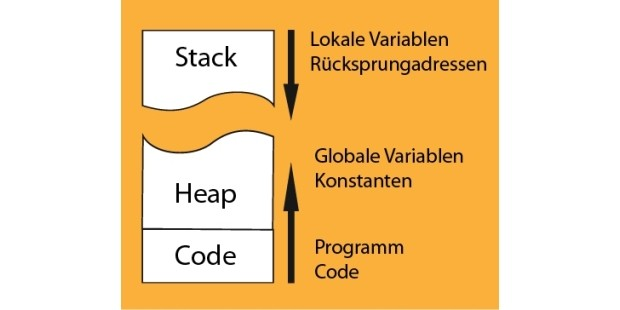
\includegraphics[width=\textwidth]{images/BufferOverflow/speicherAufbau}
	\caption{Aufbau des Speichers beim Start eines Programmes: Code -> Heap -> Stack}
	\label{fig:speicherAufbau}
\end{figure}

Für das Überschreiben der nachfolgenden Speicherbereiche ist die Speicherverwaltung verantwortlich. Beim Start eines Programmes wird diesem nämlich ein bestimmter Speicherbereich zugewiesen. Dieser ist, wie in Abbildung \ref{fig:speicherAufbau} dargestellt, in drei Abschnitte aufgeteilt: den Code, den Heap und den Stack. \\
Im Code liegt der eigentliche Quellcode, der nicht mehr verändert werden kann. Darüber liegt der Heap, in dem dynamische Variablen abgelegt sind. Der Stack beginnt am oberen Ende des Speichers und wächst mit jedem Eintrag nach unten. Dabei wird nach dem Prinzip des LIFO (last in, first out) vorgegangen. Gespeichert werden im Stack lokale Variablen, der Inhalt von Prozessorregistern und Rücksprung-Adressen von Unterprogrammen. Bei einem Angriff durch Buffer-Overflow wird einen lokale Variable mit mehr Daten beschrieben, als reserviert sind. Deshalb wird der nachfolgende Speicherbereich überschrieben, was entweder andere lokale Variablen oder aber Rücksprung-Adressen sein können.

Hier beginnt der eigentlich schädliche Angriff. Wurde zuvor bereits Schadcode auf dem Rechner des Opfers gespeichert, kann die Rücksprung-Adresse nun auf den Einsprungpunkt dieses Schadcodes zeigen. Mit Hilfe eines einfachen C-Programmes soll dies verdeutlicht werden. Darin wird zuerst ein Buffer angelegt und danach das beim Programmaufruf übergebene Argument in diesem Buffer gespeichert.

\begin{figure}
	\centering
	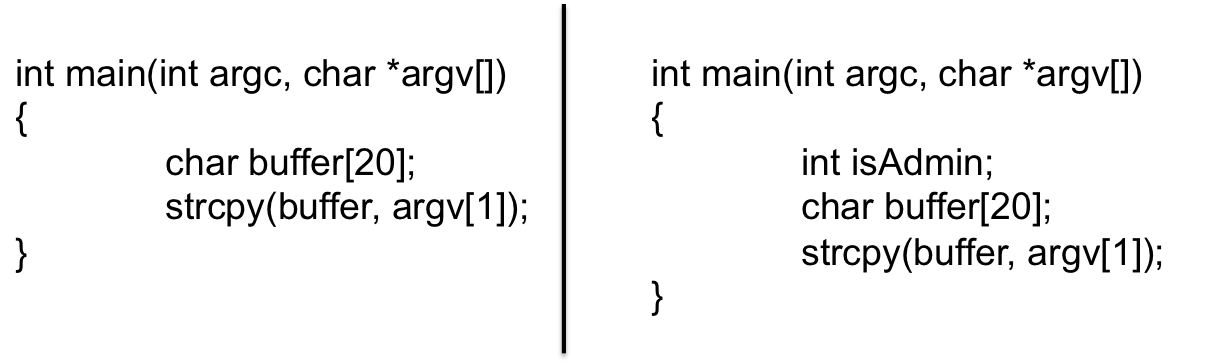
\includegraphics[width=\textwidth]{images/BufferOverflow/beispielCode}
	\caption{links: Eingabeargument wird nicht überprüft, kann aber keinen Schaden anrichten, rechts: Eingabeargument wird nicht überprüft und es ist möglich die Variable isAdmin zu überschreiben}
	\label{fig:beispielCode}
\end{figure}

In Abbildung \ref{fig:beispielCode} sind zwei kurze Programme nach diesem Aufbau gegeben. Im linken Bild kann nicht viel passieren, da nur eine Variable gespeichert wird. Im rechten Bild kann hingegen die Variable isAdmin bei zu langem Eingabeargument überschrieben werden.

Um herauszufinden, ab wann es sich um eine \enquote{zu lange} Eingabe handelt, muss der Assembler Code des Programmes analysiert werden.
Der Dump des Assembler Codes der main-Funktion auf dem rechten Teilbild sieht folgendermaßen aus:

\begin{lstlisting}
0x4004e6 <+0>: push rbp
0x4004e7 <+1>: mov rbp,rsp
0x4004ea <+4>: sub rsp,0x30
0x4004ee <+8>: mov DWORD PTR [rbp-0x24],edi
0x4004f1 <+11>:mov QWORD PTR [rbp-0x30],rsi
0x4004f5 <+15>:mov DWORD PTR [rbp-0x4],0x0
0x4004fc <+22>:mov rax,QWORD PTR [rbp-0x30]
0x400500 <+26>:add rax,0x8
0x400504 <+30>:mov rdx,QWORD PTR [rax]
0x400507 <+33>:lea rax,[rbp-0x20]
0x40050b <+37>:mov rsi,rdx
0x40050e <+40>:mov rdi,rax
0x400511 <+43>:call 0x4003c0
0x400516 <+48>:mov eax,0x0
0x40051b <+53>:leave
0x40051c <+54>:ret
\end{lstlisting}

In den ersten drei Zeilen wird der Speicher für die beiden Variablen buffer und isAdmin reserviert. In Zeile <+15> wird in den Basepointer der isAdmin-Variable 0x4 eine Null geschrieben. In Zeile <+33> wird dann die Adresse der Nutzereingabe geladen. Dabei steht "'lea"' für load effective adress. Man kann hier also ablesen, dass die Nutzereingabe der buffer-Variable bei rbp-0x20 beginnt. Soll jetzt also beim Eintragen der buffer-Variable die isAdmin-Variable überschrieben werden, sind 0x20-0x4+1 (=29) Zeichen notwending.

\section{Vorbereitung}
Notwendige Hardware:

\begin{itemize}
	\item Kali Linux 2.0 mit der Security Workbench
\end{itemize}

\section{Ablauf}
Das Tutorial besteht aus zwei einfachen Beispielen, bei denen ausgehend vom Quellcode eine Objekt-Datei erstellt und ausgewertet wird. Danach können selbstständig zwei weitere, ähnliche Aufgaben gelöst werden, bei denen lediglich die Objekt-Dateien vorhanden sind.

Zur Durchführung dieses Tutorials musst du die Security Workbench öffnen und dort die Nummer 7 \enquote{Buffer Overflow} wählen.

\subsection{Erstes Beispiel}
Wähle beim ersten Durchgang des Tutorials Nummer 1 \enquote{Erstes Beispiel}

Als Erstes musst du dir nun den Quellcode von BufferOverflow/FirstExample.c in einem Texteditor anschauen. Es werden darin zuerst drei Variablen angelegt. Im Anschluss wird das Eingabeargument in einer der Variablen gespeichert. Da das Argument vor der Speicherung nicht auf seine Größe überprüft wird, ist es möglich die anderen Variablen mit einer zu großen Eingabe zu überschreiben.

Nun soll der Quellcode in ein ausführbares Programm kompiliert werden. Dies wird mit folgendem Befehl gemacht:
\begin{lstlisting}
gcc -ggdb BufferOverflow/FirstExample.c -o BufferOverflow/FirstExample
\end{lstlisting}
(\colorbox{altgray}{\lstinline|gcc|} startet den GNU Kompiler und speichert aufgrund der Option \colorbox{altgray}{\lstinline|-ggdb <name>|} auch Informationen des angegebenen Programmes, die später mit dem GNU Debugger ausgelesen werden können, mit \colorbox{altgray}{\lstinline|-o <name>|} wird außerdem der Name angegeben unter dem die erstellte Objekt-Datei gespeichert werden soll)

\begin{figure}
	\centering
	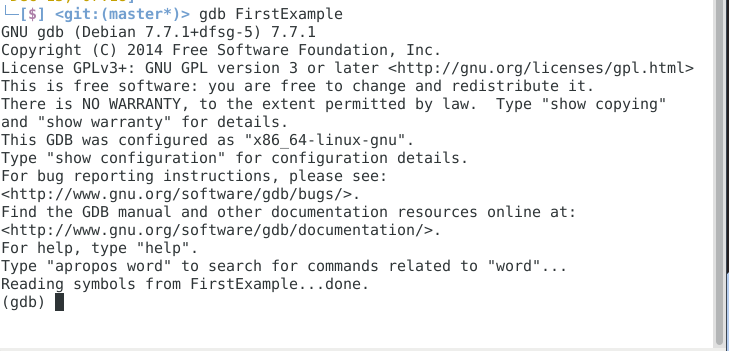
\includegraphics[width=\textwidth]{images/BufferOverflow/gnuDebugger}
	\caption{Beispiel, wie der Start des GNU Debuggers aussehen sollte}
	\label{fig:gnuDebugger}
\end{figure}

Um nun den Assembler-Code des erzeugten Programmes zu analysieren wird der GNU Debugger verwendet. Da hier ein Unterprozess geöffnet wird, startet ein neues Terminal mit dem GNU Debugger. Wie dieses aussieht, kannst du in Abbildung \ref{fig:gnuDebugger} sehen. Du kannst im ersten Terminal weiter die Befehle durchgehen und im zweiten den Assembler-Code analysieren. Gestartet wird der GNU Debugger mit dem Befehl:
\begin{lstlisting}
gdb BufferOverflow/FirstExample
\end{lstlisting}
(\colorbox{altgray}{\lstinline|gdb <name>|} startet den GNU Debugger mit der angegebenen Objekt-Datei)

Jetzt wollen wir direkt den Assembler-Code lesen, was mit folgendem Befehl möglich ist
\begin{lstlisting}
disas main
\end{lstlisting}
(\colorbox{altgray}{\lstinline|disas <name>|} startet den Disassembler der angegebenen Funktion aus dem Programm, mit dem der Debugger gestartet worden ist)

Beim Analysieren muss herausgefunden werden welche Variablen wo gespeichert werden. Dann wird ausgerechnet, wie viele Stellen das Eingabeargument benötigt, um die gewünschte Variable mit zu überschreiben. In diesem Beispiel sind es 77 Stellen: 0x50-0x4=0x4C=76 Stellen ist der Speicherplatz für das Eingabeargument. Plus eine Stelle zum Überschreiben von der Administratorvariablen.

Nach der Anaylse des Codes kann der GNU Debugger wieder geschlossen werden. Dazu wird zuerst der Disassembler geschlossen mit
\begin{lstlisting}
q
\end{lstlisting}
(\colorbox{altgray}{\lstinline|q|} schließen des Disassemblers).

Im Anschluss wird der GNU Debugger geschlossen, ebenfalls mit dem Befehl
\begin{lstlisting}
quit
\end{lstlisting}
(\colorbox{altgray}{\lstinline|quit|} schließen des GNU Debuggers)

Da das zusätzliche Terminal nun nicht mehr benötigt wird, kann es ebenfalls geschlossen werden. Das wird durchgeführt mit
\begin{lstlisting}
exit
\end{lstlisting}
(\colorbox{altgray}{\lstinline|exit|} schließt das Terminal)

Jetzt kannst du das ausführbare Programm mit folgender Eingabe auf dem Terminal starten:
\begin{lstlisting}
./BufferOverflow/FirstExample <Eingabeargument>
\end{lstlisting}
(\colorbox{altgray}{\lstinline|./<Programmname>|} damit wird ein Programm aus dem aktuellen Ordner gestartet, Eingabe kann bei Bedarf inkl. der Odnerstruktur erfolgen; \\
\colorbox{altgray}{\lstinline|<Eingabeargument>|} zusätzlich kann ein Eingabeargument zur Ausführung mit angegeben werden)

Du kannst diese Eingabe mehrmals hintereinander machen und dabei gezielt eine Überschreibung der isAdmin-Variable herbeiführen oder eine Ausführung ohne Überschreibung starten.

\subsection{Zweites Beispiel}
Wähle zur Durchführung des zweiten Beispiels Nummer 2 \enquote{Zweites Beispiel}

Als Erstes musst du dir nun den Quellcode von BufferOverflow/SecondExample.c in einem Texteditor anschauen. Es werden darin zuerst drei Variablen angelegt und im Anschluss wird das Eingabeargument in einer der Variablen gespeichert. Da das Argument vor der Speicherung nicht auf seine Größe überprüft wird, ist es möglich die anderen Variablen mit einer zu großen Eingabe zu Überschreiben.

Nun soll der Quellcode in ein ausführbares Programm kompiliert werden. Dies wird mit folgendem Befehl gemacht:
\begin{lstlisting}
gcc -ggdb BufferOverflow/SecondExample.c -o BufferOverflow/SecondExample
\end{lstlisting}
(\colorbox{altgray}{\lstinline|gcc|} startet den GNU Kompiler und speichert aufgrund der Option \colorbox{altgray}{\lstinline|-ggdb <name>|} auch Informationen des angegebenen Programmes, die später mit dem GNU Debugger ausgelesen werden können, mit \colorbox{altgray}{\lstinline|-o <name>|} wird außerdem der Name angegeben unter dem die erstellte Objekt-Datei gespeichert werden soll)

Um nun den Assembler-Code des erzeugten Programmes zu analysieren wird der GNU Debugger verwendet. Gestartet wird dieser mit dem Befehl
\begin{lstlisting}
gdb BufferOverflow/SecondExample
\end{lstlisting}
(\colorbox{altgray}{\lstinline|gdb <name>|} startet den GNU Debugger mit der angegebenen Objekt-Datei)

Jetzt wollen wir direkt den Assembler-Code lesen, was mit folgendem Befehl möglich ist
\begin{lstlisting}
disas main
\end{lstlisting}
(\colorbox{altgray}{\lstinline|disas <name>|} startet den Disassembler der angegebenen Funktion aus dem Programm, mit dem der Debugger gestartet worden ist)

Beim Analysieren müssen die zuvor angesprochenen Angaben gesucht werden. Welche Variablen werden wo gespeichert. Dann muss ausgerechnet werden, wie viele Stellen das Eingabeargument benötigt, um die gewünschte Variable mit zu überschreiben. In diesem Beispiel sind es 69 Stellen: 0x50-0x8-0x4=0x44=68 Stellen ist der Speicherplatz für das Eingabeargument. Plus eine Stelle zum Überschreiben von der Administratorvariablen.

Nach der Anaylse des Codes kann der GNU Debugger wieder geschlossen werden. Dazu wird zuerst der Disassembler geschlossen mit
\begin{lstlisting}
quit
\end{lstlisting}
(\colorbox{altgray}{\lstinline|quit|} schließen des Disassemblers).

Im Anschluss wird der GNU Debugger geschlossen, ebenfalls mit dem Befehl
\begin{lstlisting}
quit
\end{lstlisting}
(\colorbox{altgray}{\lstinline|quit|} schließen des GNU Debuggers)

Da das zusätzliche Terminal nun nicht mehr benötigt wird, kann es ebenfalls geschlossen werden. Das wird durchgeführt mit
\begin{lstlisting}
exit
\end{lstlisting}
(\colorbox{altgray}{\lstinline|exit|} schließt das Terminal)

Jetzt kannst du das ausführbare Programm mit folgender Eingabe auf dem Terminal starten:
\begin{lstlisting}
./BufferOverflow/SecondExample <Eingabeargument>
\end{lstlisting}
(\colorbox{altgray}{\lstinline|./|} damit wird ein Programm aus dem aktuellen Ordner gestartet; \\
\colorbox{altgray}{\lstinline|./<Programmname> <Eingabeargument>|} zusätzlich wird der Programmname - bei Bedarf inkl. der Ordnerstruktur - mit dem angegebenen Eingabeargument ausgeführt)

Du kannst diese Eingabe mehrmals hintereinander machen und dabei gezielt eine Überschreibung der isAdmin-Variable herbeiführen oder eine Ausführung ohne Überschreiben starten.

\subsection{Aufgaben}
Zusätzlich zu den beiden gerade erklärten Beispielen stehen zwei Aufgaben zur Verfügung. Bei diesen ist lediglich die Objekt-Datei gegeben und es soll auch hier herausgefunden werden, wie viele Stellen das Eingabeargument besitzen muss, damit das Passwort ausgegeben wird (weil man die Administratorvariable überschrieben hat).

Die Aufgaben liegen im Unterordner Projekte/BufferOverflow und heißen Buffer1 bzw. Buffer2.

\section{Gegenmaßnahmen}
\subsection{Programmierer}
Ist man selbst der Programmierer und möchte Angriffe auf den eigenen Code verhindern, ist die einfachste Methode das Benutzen von modernen Compilern in Kombination mit Visual C++ 2010-Projekten. Diese prüfen bereits beim Compilieren, ob etwa unsichere Befehle wie \enquote{strcpy} anstatt der sicheren Variante von \enquote{strcpy\_s} verwendet werden und gibt entsprechende Warnungen aus. Sollte diese Warnung ignoriert werden, so wird trotzdem ein sicherer Code erzeugt, da automatische Funktionen in den Code mit eingepflegt werden. Zu diesen Funktionen gehört die \enquote{Adress space layout randomization} (ASLR) die der Funktion bei jedem Programmstart eine neue Adresse im Speicher zuweist. Der Compiler-Schalter /GS ist eine Puffersicherheitsüberprüfung, die einen Buffer-Overflow abfängt und das Programm aufgrund des Compiler-Schalters /RTC1 (zur vollständigen Laufzeitüberprüfung) die Programmausführung abbricht.

Dass trotz all diesen Möglichkeiten noch Buffer-Overflow-Angriffe möglich sind, liegt an den alten Entwicklungsumgebungen. Viele Programme werden noch in solchen erstellt, da das Umziehen von Software auf neuer Umgebungen sehr viel Aufwand benötigt. Außerdem haben Hacker mittlerweile auch Methoden gefunden, um diese Sicherungen zu umgehen.

\subsection{Benutzer}
Als Benutzer eines Programmes ist man darauf angewiesen, dass der Hersteller seine Programme möglichst gut abgesichert hat. Durch regelmäßige Updates kann man den neuesten Schutz des Herstellers verwenden.

Eine andere Möglichkeit ist die Wahl von alternativer Software (Foxit Reader statt Adobe Reader). Hier kann man auf wenig Hacker-Angriffe hoffen, da diese normalerweise für einen großen Effekt weit verbreitete Software angreifen.

Die letzte Möglichkeit stellt das kostenloses Microsoft Tool Emet (Enhanced Mitigation Experience Toolkit) dar. Dieses sichert Programme nachträglich mit den im vorherigen Abschnitt erklärten Schutzmechanismen ab und bietet somit zumindest einen kleinen Schutz vor Angriffen.